% =============================================================================
% Introduction
% =============================================================================

\section{Introduction}
\label{sec:intro}

\begin{figure}[!t]
  \centering
  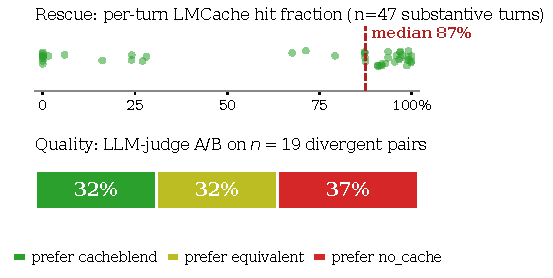
\includegraphics[width=\columnwidth]{figures/teaser.pdf}
  \caption{\sys{}'s headline finding on Llama-3.3-70B-Instruct fp8.
  Cacheblend rescues 95--99\% of post-compaction prompt tokens at the
  prefill stage (top), reproducing the published rescue numbers on
  natural Claude Code agent traffic (to our knowledge for the first
  time on this workload class). But on the
  divergent (capture, turn) pairs --- the 19 of 47 substantive pairs
  in the deep-evaluation subset where cacheblend's blended-KV output
  is not bit-identical to a no-cache baseline at $T{=}0$ --- a
  Sonnet-4.6 LLM judge prefers cacheblend's
  output on only 31.6\% of pairs and finds it non-inferior on 63.2\%
  (bottom), well below the design specification's 85\% gate.
  Hit rate is not output quality.}
  \label{fig:teaser}
  \Description{Two horizontal bars stacked vertically. Top bar shows a
  green segment at 95 to 99 percent on a gray 0 to 100 percent axis,
  labeled "Rescue: post-compaction prefill tokens served from cache".
  Bottom bar shows a stacked horizontal bar with three segments:
  prefer cacheblend at 32 percent in green, equivalent at 32 percent
  in olive, and prefer no_cache at 37 percent in red, labeled
  "Quality: LLM-judge A/B on n=19 divergent pairs".}
\end{figure}

Large language model serving has converged on a layered KV-cache
architecture: vLLM~\cite{vllm-sosp} provides paged-attention prefix
caching within a session, and LMCache~\cite{lmcache-paper} extends it
to a cross-request CPU-resident store. These mechanisms cleanly handle
the common case where requests share an exact textual prefix
(retrieval-augmented generation, fixed system prompts, etc.). They
\emph{cannot} handle the case where two requests share \emph{most} of
their tokens but differ in a chunk near the front --- the textbook
cacheblend~\cite{lmcache-cacheblend} use case --- without recomputing
the entire suffix.

Modern agent harnesses sit precisely in that gap. Claude
Code~\cite{claude-code} (CC), the deployment we study, drives an
LLM through long multi-turn task sessions: a single SWE-bench Verified
task averages 5\,turns at 5\,k--10\,k prompt tokens each, and a typical
half-day session routinely crosses 100\,k tokens before triggering
CC's built-in \texttt{/compact} summarization. \texttt{/compact}
replaces most of the conversation history with a roughly 800-token
summary --- which, by construction, breaks the prefix-match invariant
that prefix caching depends on. \emph{Every} post-compaction request
re-prefills nearly from scratch on existing caches.

\paragraph{Cacheblend's promise and its production gap.}
Cacheblend~\cite{lmcache-cacheblend} proposes a \emph{selective KV
recompute} strategy: chunk a request's tokens by a special separator,
retrieve cached KV blocks for the chunks that match, and recompute KV
only for a configurable fraction (default 15\%) of the chunks that
have shifted positionally. The published evaluation shows
70--90\,\%~hit rates on permuted RAG retrieval workloads, where
chunked retrieval is the design pattern users already write toward.
Adapting cacheblend to CC traffic, however, exposes three integration
issues that prior work does not address:

\begin{enumerate}
\item \textbf{Chunk-boundary mismatch.} On lmcache v0.4.2 against
vLLM v0.19.0, the \texttt{STORE} path hashes a chunk-aligned token range
($\lfloor n/256 \rfloor \cdot 256$) while the \texttt{LOOKUP} path hashes the full
prompt range ($n$). Store and lookup hashes never agree, retrieval rate
is 0\% regardless of how the workload is shaped.
\item \textbf{Per-turn hash drift.} CC's \texttt{x-anthropic-billing-header}
embeds per-turn fields (\texttt{cch=}, a chunk hash; \texttt{cc\_version=},
the CC binary version) into the first KV chunk. Within a single
multi-turn session, these change between turns, so chunk 0's hash is
distinct on every request --- cache hits do not propagate even when the
rest of the prompt is identical.
\item \textbf{No structural separators.} Cacheblend's segment detector
requires its configured \texttt{blend\_special\_str} (default \texttt{\#\,\#})
to appear at chunk boundaries. CC's outbound traffic uses \texttt{\textbackslash n\textbackslash n}, which
tokenizes to 25--180 tokens per segment --- below cacheblend's 256-token
\texttt{blend\_min\_tokens} floor. The segment detector finds zero
chunks; cacheblend never engages.
\end{enumerate}

\paragraph{The output-quality question.}
A second gap is methodological. Cacheblend's published numbers are
expressed in cache-byte hit rate. But the system's value proposition
ultimately rests on the assumption that the rescued KV produces
\emph{the same output} as the all-fresh-compute baseline. Selective
KV recompute is, by construction, an approximation: the recomputed
chunks see different positional and attention context than the
original compute pass. The cacheblend paper~\cite{lmcache-cacheblend}
notes ``small but bounded quality drift'' but does not quantify it on
agent workloads, where a single-token difference between a tool-call
JSON block and natural-language prose can be the difference between
agent progress and a stalled task.

\paragraph{Contributions.} This paper makes three contributions:

\begin{enumerate}
\item \textbf{A working integration of cacheblend with real Claude Code
traffic} (\S\ref{sec:system}). We present three patches addressing the
integration issues above and show, on a Llama-3.3-70B-Instruct fp8
backend with tensor-parallelism, a median 76.5\% rescue rate over
$n{=}99$ substantive turns across two \dataset{} subsets, with a 6\%
mass of turns achieving the published 95--99\,\% steady-state peak
on long-prompt SWE-V traffic and 0\% on the
\texttt{skill\_invocation/} workload.

\item \textbf{\dataset, a reproducible public benchmark}
(\S\ref{sec:benchmark}) of 13 redacted real Claude Code captures
spanning 182\,turns and 411\,k total tokens across 5\,SWE-bench
Verified tasks, a skill-invocation capture covering 5\,skills
$\times$\,3\,prompts, and 7\,post-\texttt{/compact} multi-turn
diagnostic captures, published under CC-BY 4.0 on Hugging
Face~\cite{claudecode-trace-hf}.

\item \textbf{To our knowledge, the first measurement of cacheblend's agent-protocol
usefulness cost on natural agent traffic} (\S\ref{sec:evaluation}).
At $T=0$, cacheblend produces bit-identical output to no\_cache on 57\%
of substantive turns and severe ($<$0.3 token-identity) divergence on
30\%, including 11\% with decode-mode flips. A Sonnet-4.6 LLM-judge
blind A/B over the divergent pairs prefers cacheblend on 32\% (95\%
Wilson CI [15\%, 54\%]) and finds cacheblend conditionally non-inferior
on 63\% (end-to-end non-inferiority across all substantive turns is
85\%, just clearing the 85\% spec gate when bit-identical pairs are
counted as guaranteed equivalents).
\end{enumerate}

We close with a discussion of what this means for production deployment
(\S\ref{sec:discussion}): cacheblend's rescue is real but not free, and
systems papers should report quality alongside hit rate.

